\section{Manuale GUI}
Nel caso in cui i file non venissero trovati viene visualizzato un messaggio informativo. Dopo aver inserito le credenziali, se corrette, l'utente visualizza la finestra principale dalla quale se è di tipo admin può accedere alla gestione dei tavoli e degli utenti dalla barra del menu, altrimenti può effettuare il logout oppure cambiare i propri dati personali dopo aver selezionato l'opzione "\textbf{Opzioni}" dalla barra del menu.
L'admin può accedere alle funzioni di modifica cliccando due volte sopra la riga dell'oggetto su cui intende effettuare le modifiche:
\clearpage
\begin{figure}[!h]
\centering
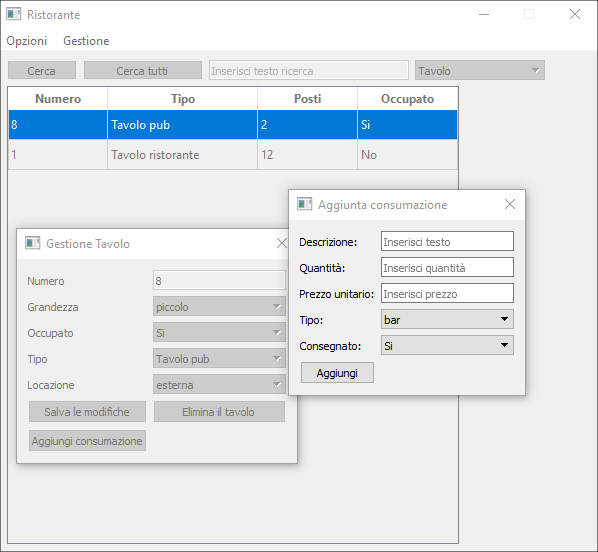
\includegraphics[scale=0.60]{res/sections/immagini/gui.png}
\caption{View gestione tavoli di un utente admin}
\end{figure}

Per gli utenti camerieri questa funzionalità è prevista solo per la modifica e l'eliminazione delle consumazioni, che può essere effettuata cliccando due volte sopra la riga della consumazione effettuata per eliminarla e/o modificarla mentre per l'aggiunta di una consumazione sarà necessario cercare il tavolo a cui si vuole aggiungere una consumazione e cliccare due volte sopra di esso.

Per gli utenti di tipo cuoco queste funzionalità non sono presenti, essi possono effettuare unicamente ricerche.
La ricerca di un utente avviene per username oppure si possono visualizzare tutti gli utenti.
La ricerca di un tavolo avviene per numero oppure si possono visualizzare tutti i tavoli.
La ricerca di una consumazione avviene per numero tavolo oppure digitando la descrizione di una consumazione che si vuole ricercare o parte di essa; la ricerca di una descrizione vuota equivale alla ricerca di tutte le consumazioni.

Nell'inserimento dei dati utente vengono fatti alcuni controlli con espressioni regolari al fine di permettere l'inserimento di sole lettere nei campi \textbf{nome}, \textbf{cognome}, per \textbf{username} è permesso l'inserimento anche di numeri, mentre per \textbf{password}  non avvengono controlli.

Nell'inserimento dei dati tavoli vengono fatti alcuni controlli con espressioni regolari al fine di permettere l'inserimento di soli numeri nei campi \textbf{numero} e \textbf{piano}.

Nell'inserimento dei dati consumazioni vengono fatti alcuni controlli con espressioni regolari al fine di permettere l'inserimento di sole lettere nel campo \textbf{descrizione}, per \textbf{quantità} è permesso l'inserimento di soli numeri, mentre per \textbf{prezzo} è permesso l'inserimento di numero con al massimo due cifre decimali.

\clearpage
	